\section{Symmetric Matrices}

Recall matrix $A$ is symmetric if $A=A^\intercal$ and orthogonal if $A^\intercal = A^{-1}$.

\begin{definition}
  \textbf{Real Symmetric Matrix}: If $A$ is a real symmetric matrix:
    \begin{enumerate}
      \item Eigenvalues of $A$ are real.
      \item Eigenvectors of $A$ corresponding to district eigenvalues are orthogonal to each other.
      \item $A$ is always diagonizable; in fact, $Q^{-1}AQ=\Lambda$ is diagonal for some orthogonal matrix $Q$ so $Q^{-1}AQ=\Lambda$ or $A=Q \Lambda Q^\intercal$. That is, $A=Q \Lambda Q^{-1}=Q \Lambda Q^\intercal$
    \end{enumerate}
\end{definition}

\begin{figure}[h]
\caption{Sample Figure}\label{figure}
\begin{center}
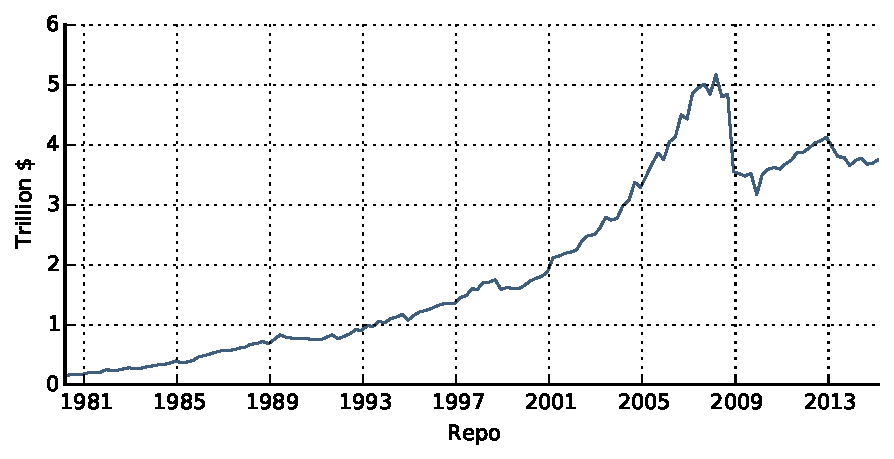
\includegraphics[width=.5\textwidth]{sample.pdf}
\end{center}
\end{figure}

\begin{example}
  We can see these properties hold for real symmetric matrices. For example:
  $A = \begin{bmatrix}[rrr]
   2 & 1 \\
   1 & 2 \\
  \end{bmatrix}$. Going through the normal process to find eigenvalues and eigenvectors we find:
  \[\lambda_1=1 \rightarrow x_1= \begin{bmatrix}[rrr]
    1 \\
    -1 \\
   \end{bmatrix}, \lambda_2=3 \rightarrow x_2= \begin{bmatrix}[rrr]
    1 \\
    1 \\
   \end{bmatrix}\]
  Thus the $\lambda's$ are real and the eigenvectors are orthogonal to each other. We can make them unit vectors to produce $Q$ which can diagonalize $A$:
  \[Q=\frac{1}{\sqrt{2}} \begin{bmatrix}[rrr]
    -1 & 1 \\
    1 & 1 \\
  \end{bmatrix} \rightarrow A: A=Q\Lambda Q^{-1}=Q\Lambda Q^\intercal \text{ with } \Lambda = \begin{bmatrix}[rrr]
   1 & 0 \\
   0 & 3 \\
 \end{bmatrix} \]
\end{example}

In other examples, the biggest problem will be that the eigenvectors won't be orthogonal to each other, e.g. $x_1 \perp x_2 $ but not $x_1, x_2 \perp x_3$, which tends to happen with repeated eigenvalues. This is fixable with the Gram-Schmidt process, though.

We will now prove the 3 key facts of real symmetric matrices (mentioned above):
\begin{enumerate}
  \item Eigenvalues of $A$ are real.
  \item Eigenvectors of $A$ corresponding to district eigenvalues are orthogonal to each other.
  \item $A$ is always diagonizable; in fact, $Q^{-1}AQ=\Lambda$ is diagonal for some orthogonal matrix $Q$ so $Q^{-1}AQ=\Lambda$ or $A=Q \Lambda Q^\intercal$. That is, $A=Q \Lambda Q^{-1}=Q \Lambda Q^\intercal$
\end{enumerate}

\subsection{Prove eigenvalues of a real symmetric matrix are real.}

\begin{proof}
    Eigenvalues of a real symmetric matrix are real.

    First we need to mention complex numbers. Recall complex numbers take the form $x+iy$ with $x,y$ real.

    \begin{definition}
        \textbf{Complex Conjugate}: if $z=x+iy$ then its complex conjugate is $ \overline{z}=x-iy$. Some useful properties of complex conjugates:
        \begin{itemize}
            \item $\overline{z+w}= \overline{z}+ \overline{w}$
            \item $\overline{zw}= \bar{z} \bar{w}$
            \item $z \overline{z}=|z|^2$
            \item $z$ is real iff $z= \overline{z}$ (i.e. $0i$)
            \item You can ``complex conjugate'' a matrix by replacing each value with its complex conjugate
            \item Then, $ \bar{A} \bar{B}=\overline{AB}$
        \end{itemize}
    \end{definition}

    Also note that for vector $x=\begin{bmatrix}[r]
     x_1 \\
     \vdots \\
     x_n
    \end{bmatrix},  \overline{x}^\intercal x = [ \overline{x_1} \dots  \overline{x_n}] \begin{bmatrix}[r]
     x_1 \\
     \vdots \\
     x_n
 \end{bmatrix} =  \overline{x_1}x_1+\dots  \overline{x_n}x_n=|x_1|^+\dots|x_n|^2=||x||^2$ which is greater than 0 unless each entry is also 0.

Goal: Show $\lambda = \bar{\lambda}$

Let A be a real, symmetric $n \times n$ matrix, thus $A=A^T$ and $A=\bar{A}$.

First: $Ax=\lambda x \rightarrow \bar{A}\bar{x}=\bar{\lambda}\bar{x} = A\bar{x}=\bar{\lambda}\bar{x} \rightarrow \bar{x}^TA=\bar{\lambda}\bar{x}^T \rightarrow  \bar{x}^TAx=\bar{\lambda}\bar{x}^Tx$

Second: $Ax=\lambda x \rightarrow \bar{x}^TAx=\bar{x}^T\lambda x$

Thus we see the left hand sides are equal, therefore the right sides are equal. They multiple $\bar{x}^Tx =$ length squared with is greater than zero. Thus $\bar{\lambda}=\lambda$ and $a+ib=a-ib$ with imaginary part $b=0$. Can do a similar process for Hermitian matrix remembering that $(Ax)^T = x^TA^T$
\end{proof}


\subsection{Prove eigenvectors of a real symmetric matrix corresponding to district eigenvalues are orthogonal to each other.}

\begin{proof}
    Eigenvectors of a real symmetric matrix corresponding to district eigenvalues are orthogonal to each other.

    Let $A$ be a real, symmetric matrix so its eigenvalues are real. If $\lambda,  \mu$ are eigenvalues for $A, \lambda \neq \mu$ with real eigenvectors $x,y$. We want to show that $x \perp y$.
    \[Ax=\lambda x \rightarrow x^\intercal A^\intercal = \lambda x^\intercal \rightarrow x^\intercal A = \lambda x^\intercal (A^\intercal=A) \rightarrow \overbrace{x^\intercal Ay=\lambda x^\intercal y}^{1}\]
    \[Ay = \mu y \rightarrow \overbrace{x^\intercal Ay= x^\intercal \mu y}^{2} \]
Now combining the highlighted relationships:
    \[ \lambda x^\intercal y = \mu x^\intercal  y \rightarrow (\lambda - \mu)x^\intercal y =0 \text{ and we know } \lambda - \mu \neq 0 \rightarrow x^\intercal y = 0 \therefore x \perp y\]
\end{proof}

\subsection{Prove a real symmetric matrix is always diagonizable.}

\begin{proof}
    A real symmetric matrix is always diagonizable.

    This proof comes from \textbf{Schur's Theorem}: If $A$ is a real $n \times n$ matrix with real eigenvalues then $A=QTQ^{-1}$ with $Q$ orthogonal [($QQ^\intercal = I) \rightarrow (Q^{-1}=Q^{\intercal})]$, and $T$ is an upper triangular matrix. Thus this is a triangularizing theorem, not diagonalizing.\footnote{There is a more general treatment which eliminates the awkward real statement we're requiring now.} $T=Q^{-1}AQ \rightarrow T=Q^\intercal AQ \rightarrow T^\intercal = (Q^{-1}AQ)^\intercal = Q^\intercal A^\intercal Q \rightarrow Q^\intercal A Q = T,$ thus $T =T^\intercal \rightarrow T$ is an upper triangular matrix, meaning it has 0's below diagonal and is also symmetric (so below diagonal = above diagonal =0's) $\rightarrow \therefore T$ is diagonal.
\end{proof}

\begin{example}
    We've already seen $A$ is not diagonizable: $A=\begin{bmatrix}[rrr]
     2 & 1 \\
     -1 & 0 \\
   \end{bmatrix}$ because $\lambda_1 = \lambda_2=1$. But we can use Shur's theorem to help. The process is to find the first eigenvector, then find a second orthogonal vector to the first (this vector probably will not be an eigenvector of $A$, but that's okay), then make orthogonal matrix $Q$ with these two vectors as usual and then solve for $T$ using $T=Q^{-1}AQ=Q^{\intercal}AQ$. Thus we get:
   \[ T=Q^{-1}AQ=Q^{\intercal}AQ \rightarrow \frac{1}{2}
   \begin{bmatrix}[rrr]
    1 & -1 \\
    1 & 1 \\
  \end{bmatrix}
  \begin{bmatrix}[rrr]
   2 & 1 \\
   -1 & 0 \\
 \end{bmatrix}
 \begin{bmatrix}[rrr]
  1 & 1 \\
  -1 & 1 \\
\end{bmatrix}
  =  \begin{bmatrix}[rrr]
    1 & 2 \\
    0 & 1 \\
\end{bmatrix} \]
which is clearly triangular.
  For a $3 \times 3$ matrix we'd get an orthogonal $Q$ such that the bottom right $2 \times 2$ minor which would then need to go through the process again. Main point: this is laborious and requires doing it twice.
\end{example}

\begin{definition}
    \textbf{Hermitian Matrix}: a matrix in which $A=\bar{A}^\intercal$ is a Hermitian matrix.
    \begin{itemize}
        \item If $A=\bar{A}^\intercal \rightarrow A$ is diagonizable and $A=Q\Lambda Q^{-1}$ with $\Lambda$ a real diagonal matrix with eigenvalues (so same as before!), and $Q^{-1}=\bar{Q}^\intercal$ where $Q$ is a \textbf{unitary matrix}.
        \item This is the true general form of what we've seen, as the conjugate has no impact if $A$ is real. (!)
    \end{itemize}
\end{definition}

\section{Positive Definite Matrices}

Recall that a real symmetric matrix $A$ has 3 important properties
\begin{itemize}
    \item $A$ has real eigenvalues.
    \item Eigenvectors for distinct eigenvalues of $A$ are orthogonal.
    \item $A$ is diagonizable.
\end{itemize}

\begin{definition}
    \textbf{Positive Definite Matrix}: A real symmetric matrix $A$ is positive definite iff $x^\intercal A x > 0$ for every nonzero $x$.
\end{definition}

\begin{example} Why do we care? Let's see an example.

\textbf{1 variable}: $f(x)$ has a local minimum if:
\begin{enumerate}
    \item $f'(x)=0,$ and
    \item $f''(x)=\frac{d^2f}{dx^2}>0$.
\end{enumerate}

\textbf{2 variables}: $f(x,y)$ has local minimum if:
    \begin{enumerate}
        \item $ \frac{\delta f}{\delta x} = \frac{\delta f}{\delta y} = 0,$ and
        \item $\begin{bmatrix}[rrr]
         \frac{d^2f}{dx^2} & \frac{d^2f}{dxdy} \\
         \frac{d^2f}{dxdy} & \frac{d^2f}{dy^2}  \\
     \end{bmatrix}$ is positive definite.
    \end{enumerate}
\end{example}

\subsection{Positive Definite Tests}

How do we test whether a given matrix $A$ is positive definite? 4 ways:
\begin{theorem} A real symmetric matrix $A$ is positive definite if any of the following holds:
\begin{enumerate}
    \item $x^\intercal A x > 0$ for all nonzero vectors $x$.
    \item All eigenvalues of $A$ are $> 0$.
    \item All pivots of $A$ are $>0$ with no row swaps allowed.
    \item If the top left $k \times k \det >0$ for $k=1,2, \dots n$.
    \subitem For example; $\begin{bmatrix}[rrr]
     a & b \\
     b & c  \\
 \end{bmatrix}$ is positive definite iff: $a>0$ (first top left determinant) and $ac-b^2>0$ (second top left determinant).
\end{enumerate}
\end{theorem}

A few examples are provided below:

\begin{example}
    Is $A$ positive definite?
    \[A=\begin{bmatrix}[rrr]
     2 & 1 \\
     1 & 1  \\
 \end{bmatrix}\]

 Yes. Using rule (4) above; $2>0$ and $(2)(1)-(1)>0 \rightarrow \therefore A$ is positive definite.

\end{example}

\begin{example}
    For which values of $c4$ is $A$ positive definite?
    \[A=\begin{bmatrix}[rrr]
     2 & 1 & 0 \\
     1 & 2 & 1  \\
     0 & 1 & c  \\
 \end{bmatrix}\]

 Eliminate to:
 \[=\begin{bmatrix}[rrr]
  2 & 1 & 0 \\
  0 & \nicefrac[]{3}{2} & 1  \\
  0 & 0 & c- \nicefrac[]{2}{3}  \\
\end{bmatrix}\]
    By rule (3) above, if $c>\frac{2}{3}$ then $A$ is positive definite.
\end{example}

\begin{example}
    Is  $A$ positive definite?
    \[A=\begin{bmatrix}[rrrrr]
     2 & 1 &  & &   \\
     1 & 2 & 1 & &    \\
      & 1 & 2 & 1 &   \\
      & \dots & \dots & \dots & \dots  \\
      & \dots & 1& 2 & 1 \\
 \end{bmatrix}\]
    Eliminate without row swaps and use rule (3) above. The matrix after elimination is an upper triangle, and the bottom right most element is $\frac{n+1}{n}$. Therefore, by rule (3) the matrix is positive definite becuase all the pivots, including $\frac{n+1}{n}, >0$.
\end{example}

It is not difficult to show that these four rules are equivalent, and are discussed in the handnotes in further detail. I'm skipping them now though.



\section{Similar Matrices}

\begin{definition}
    \textbf{Similar matrix}: Let $A, B$ be $n \times n$ matrices. $A$ is similar to $B$ if we can find an invertible matrix $M$ so that $B=M^{-1}AM$. If $A$ is similar to $B$:
    \begin{enumerate}
        \item $A,B$ have the same eigenvalues (including reptitions)
        \item $A,B$ usually don't have the same eigenvectors
    \end{enumerate}
\end{definition}

\begin{proof}
    Show if $A,B$ similar then they have the same eigenvalues.

    Suppose $B=M^{-1}AM: M^{-1}(A-\lambda I)M=M^{-1}AM-\lambda M^{-1} I M = B-\lambda I$. Take determinants: $|B-\lambda I | = |M^{-1} (A -\lambda I)M| \rightarrow \text{ recall } |AB|=|A| |B| \rightarrow |B-\lambda I | = |M^{-1}| |A -\lambda I| |M| = |A -\lambda I|$. Thus if $A,B$ similar then $|B-\lambda I | =|A-\lambda I |$ so their characteristics polynomials are the same, therefore they have the same eigenvalues with the same algebraic multiplicity (so includes repetitions).
\end{proof}

\begin{proof} What about eigenvectors?

Suppose $x$ is an eigenvector for $A$ with eigenvalue $\lambda$, and suppose $B=M^{-1}AM$. We know $\lambda$ is an eigenvalue for $B$, but what about $x$?

First rewrite $B=M^{-1}AM \rightarrow A=MBM^{-1} \rightarrow Ax=\lambda x = MBM^{-1}x = \lambda x \rightarrow B(M^{-1}x)=M^{-1}\lambda x \rightarrow B(M^{-1}x)=\lambda (M^{-1}x) \rightarrow \therefore y=M^{-1}x$ is an eigenvector of B.

Note: $y$ is nonzero $(y =M^{-1}x \neq 0)$ since $x$ is nonzero and $M^{-1}$ is invertible.

Therefore, similar matrices share the same eigenvalues but not necessarily the same eigenvectors.

\end{proof}

\subsection{Facts about similar matrices}

The following are key facts about similar matrices. If $A$ similar to $B$:
\begin{enumerate}
    \item If $A$ similar to $B$, and $B$ similar to $C$, then $A$ similar to $C$.
    \item If $A$ similar to $B$ (using $M$), then $B$ similar to $A$ (using $M^{-1}$).
    \item $A$ is always similar to $A$, (use $M=I$).
    \item If $A$ is diagonizable with eigenvalues $\lambda_1, \dots \lambda_n$ (including repteitions) then $A$ is similar to $\Lambda$, a diagonal matrix (like we've already seen, with eigenvalues on the diagonal). Then $A=S\Lambda S^{-1}$ where $S$ is an eigenvector matrix. Just like we've seen before.
    \item If $A, B$ similar and $A$ diagonizable then $B$ is diagonizable. ($B$ similar to $A$, $A$ similar to $\Lambda$, then $B$ similar to $\Lambda$ and therefore diagonizable).
    \item If $A,B$ both diagonizable with the same eigenvalues then $A, B$ are similar. So check if they have the same eigenvalues to see if similar.
\end{enumerate}

\begin{remark}
What about nondiagonizable matrices? You can use the next best thing, a \textbf{Jordan Block}. But I won't cover this now.
\end{remark}

\section{Markov Matrices}

 \begin{definition} $A$ is a \textbf{Markov matrix} if
     \begin{enumerate}
         \item all entries of $A \geq 0$ and
         \item the sum of any column of $A =1$.
     \end{enumerate}
\end{definition}

\begin{theorem}
    If $A$ is a positive Markov matrix (i.e. all entries $>0$, each column adds to 1), then $\lambda_1=1$ is larger than any other eigenvalue. The eigenvectors $x_1$ corresponding to $\lambda_1$ is the steady state.
\end{theorem}

An example will clarify.

\begin{example}
    For example, if you have two cable companies, $x,y$; suppose each month 20 percent of $x$'s customers switch to $y$, and 5 percent of $y$'s customers switch to $x$ (assuming nobody entering or exiting). What happens in the long run. The beginning fraction with company $x$ is 2\%.

    If we say that $u_0$ is the starting vector, we can see how this changes over time after multiplying by itself many times:
    \[A =  \begin{bmatrix} 0.8 & 0.05  \\  0.2 & 0.95 \end{bmatrix} , u_1=Au_0 \rightarrow u_2=Au_1=A^2u_0\]
    After $k$ steps we will have $A^ku_0$. Thus these vectors, $u_1,u_2 \dots$ approach a steady state. We want to find a steady state such that:
    \[\begin{bmatrix} 0.8 & 0.05  \\  0.2 & 0.95 \end{bmatrix} x = x\]

    Now we will solve for the steady state:
    \begin{enumerate}
        \item Find the eigenvalues. A Markov matrix always has an eigenvalue of 1, and the other can be derived from the trace (the sum of the diagonals) as we know the sum of the eigenvalues = the trace. Thus $\lambda_1=1, \lambda_2=0.75$.
        \item Find the eigenvectors. This is the normal process.
        \[\lambda_1=1: x_1=\begin{bmatrix}[rrrrr] 0.2  \\  0.8 \end{bmatrix}, \lambda_2=0.75: x_2=\begin{bmatrix}[rrrrr] 1  \\  -1 \end{bmatrix} \]
        \item Now diagonalize and solve:
        \[u_k=A^nu_0 \text{ and } A^n=S \Lambda^n S^{-1} \rightarrow u_k=S \Lambda^n S^{-1}u_0\]
        \[u_k = \begin{bmatrix}[rrrrr] 0.2  & 1 \\  0.8 & 1 \end{bmatrix}
        \begin{bmatrix}[rrrrr] 1  & 0 \\  0 & 0.75 \end{bmatrix}
            \begin{bmatrix}[rrrrr] 1  & 1 \\  0.8 & -0.2 \end{bmatrix}
                \begin{bmatrix}[rrrrr] 0.02 \\  0.98 \end{bmatrix}=
                    \begin{bmatrix}[rrrrr] 0.2 \\  0.8 \end{bmatrix}\]
        \item So the eigenvector with $\lambda=1$ is the steady state.
    \end{enumerate}
\end{example}

\begin{theorem} If $A$ is Markov and all entries $>0$ then
\begin{enumerate}
\item $\lambda_1 = 1$ is an eigenvalue of $A$ (also true of all entries are $\geq 0$.)
\item If $\lambda_1$ is any other value, then $|\lambda|<1$.
\item For eigenvalue $\lambda_1 = 1$ there's a unique eigenvector $v_1$ (normalized so sum of components is 1).
\item All components of $v_1$ are positive.
\item $v_1$ is unique steady state: for any vector $u_k, A^ku_0\rightarrow cv_1$ where $c$ is sum of components of vector $u_0$.
\end{enumerate}
\end{theorem}

So in Markov matrices, if eigenvalues are distinct $\rightarrow$ $A$ is diagonizable $\rightarrow$ eigenvectors are linearly independent and importantly form a basis in $R^n$. Then you can find the eigenvector for $\lambda = 1$.

\section{What About Non-Diagonizable Matrices? Jordan Blocks}
What's the best that can be done?
\begin{definition} A $k \times k$ \textbf{Jordan Block} with eigenvalue $\lambda$ is $J\begin{bmatrix}
    \lambda_1 & 1 & \hdots \\  & \lambda_2 & 1 & \hdots \\ & & \lambda_3 & 1 & \hdots\\  \vdots \\
\end{bmatrix}$ where $\lambda$ is the only eigenvalue of $J$.
\end{definition}

Therefore, $J-\lambda I = \begin{bmatrix}
    0 & 1 & \hdots \\  & 0 & 1 & \hdots \\ & & 0 & 1 & \hdots\\  \vdots \\
\end{bmatrix}$

Then: $(J-\lambda I)x = \begin{bmatrix}
    0 & 1 & \hdots \\  & 0 & 1 & \hdots \\ & & 0 & 1 & \hdots\\  \vdots \\
\end{bmatrix} \begin{bmatrix}
    x_1 \\  \vdots \\ \vdots \\  x_k \\
\end{bmatrix} = 0$. So all eigenvectors of $J$ are multiples of  $\begin{bmatrix}
    1 \\  0 \\ \\ \vdots \\  0 \\
\end{bmatrix}$

$J$ is not diagonizable if $k>1$, eigenvalue $\lambda$ has geometric multiplicity 1 (and only 1 linear independent eigenvector).

\begin{theorem} Every $n \times n$ matrix $A$ is similar to a \textbf{Jordan Form} $\begin{bmatrix}
    J_1 & \hdots \\  & J_2 & \hdots \\ & & J_3 & 1 & \hdots\\  \vdots \\
\end{bmatrix}$ where $J_1 \hdots J_2$ are Jordan Blocks for eigenvalues $\lambda_1, \hdots , \lambda_s$ of $A$.
\end{theorem}

Note: Not going to learn how to reduce A to a Jordan Block.

Jordan Form for A is unique (except reordering blocks).

For example, every $3 \times 3$ matrix with eigenvalues 3,3,3 is similar to one and only one of:
\begin{enumerate}
\item $\begin{bmatrix}
    3 & 0 & 0  \\   0 & 3 & 0 \\  0 & 0 & 3
    \end{bmatrix}$ If the matrix is diagonizable, with geometric multiplicity 3.
\item $\begin{bmatrix}
    3 & 0 & 0  \\   0 & 3 & 1 \\  0 & 0 & 3
    \end{bmatrix}$ with a $2 \times 2$ Jordan Block, $J$, in the bottom right corner, with geometric multiplicity 2.
\item $\begin{bmatrix}
    3 & 1 & 0  \\   0 & 3 & 1 \\  0 & 0 & 3
    \end{bmatrix}$ with a $3 \times 3$ Jordan Block, $J$ with geometric multiplicity 1.
\item Note that none of these are similar to each other.
\end{enumerate}
